\chapter{Design And Implementation Of Embedded Code Service}

Based on the analysis conducted in the previous chapter, we now have a clear understanding of what Embedded Code Service is, what is its purpose and how it is going to solve the outlined problems. In this chapter, we are going to introduce and reason about its design. We are also going to explain what changes need to be done to programming language scanners in order for them to be integrated with Embedded Code Service. At the end of the chapter we will present interesting parts of the implementation based on this design.

\section{Embedded Code Service design}

Firstly, let us summarize the steps that Embedded Code Service has to execute, because it might not be clearly obvious from previous chapters. The goal of the service is to perform data flow analysis of embedded code using one of the already existing scanners to create a data lineage graph of that code which will then be merged with the graph produced by a source technology scanner. A programming language scanner works in three steps: extraction of the input, data flow analysis and generating Manta graph. Embedded Code Service needs to perform input orchestration using the provided configuration, then launch all three stages of a scanner and after that, help to merge the graphs. The workflow looks as follows (active components are written in parentheses):
\begin{enumerate}
    \item Input orchestration (Embedded Code Service)
    \item Input extraction (scanner's Extractor)
    \item Data flow analysis (scanner's Reader)
    \item Generating lineage graph (Intermediate Dataflow Generator)
    \item Merging graphs (source technology scanner with the help of Embedded Code Service)
\end{enumerate}

\subsection{Multiple programming languages}

The first decision we have to make is whether we want to implement one universal service that can analyze embedded code written in any programming language or whether we want to have specific implementations for each programming language. This decision will greatly influence how the interface of the service is designed.
\par
An initial idea seems to be a universal service, because that is how Dataflow Query Service is implemented. A common service promotes code reuse as multiple parts of the problem will be solved in a similar way regardless of used programming language and data technology, such as merging the graphs of embedded code and source technology. We can also find similarities between the data technologies (e.g., stored procedures written in embedded code in databases) regardless of the programming language used. One service also means that only one component will need to be maintained. The downside of having one service is that its interface needs to be universal, so if one programming language has a different requirement or requires a specific modification, these changes will have to be reflected for other programming languages as well.
\par
One could argue that another benefit of one service is that we have access to the analysis of any embedded code we may find, but that turns out not to be as beneficial as it may sound. In reality, the language of embedded code is always known, so it is easy to use a specific service to analyze it. Having a universal service is crucial in case of Dataflow Query Service, because it supports recognition of the SQL dialect used in the query, but in case of Embedded Code Service such feature is not needed. When implementing specific services, we can still reach similar code reuse by grouping common logic in base classes, which makes one less argument in favor of a common service. An important advantage that multiple services provide is that they not only allow the interfaces to be tailored to the needs of the programming language scanner, but they also allow different development pace for each service. The fact is that a service for Python is much more preferred by the stakeholders because of its potential and thus a lot more resources are dedicated to working on it.
\par
Comparing the two approaches, we chose specific implementations as a more suitable solution.
The last argument carries great significance due to its profound impact on the development process, so we decided to implement multiple services, each dedicated for one programming language.  
\par
Figure~\ref{fig:ECSbasedesign} shows how a specific service processes embedded code as well as components that is utilizes. The diagram is generic for any programming language.

\begin{figure}[ht]\centering
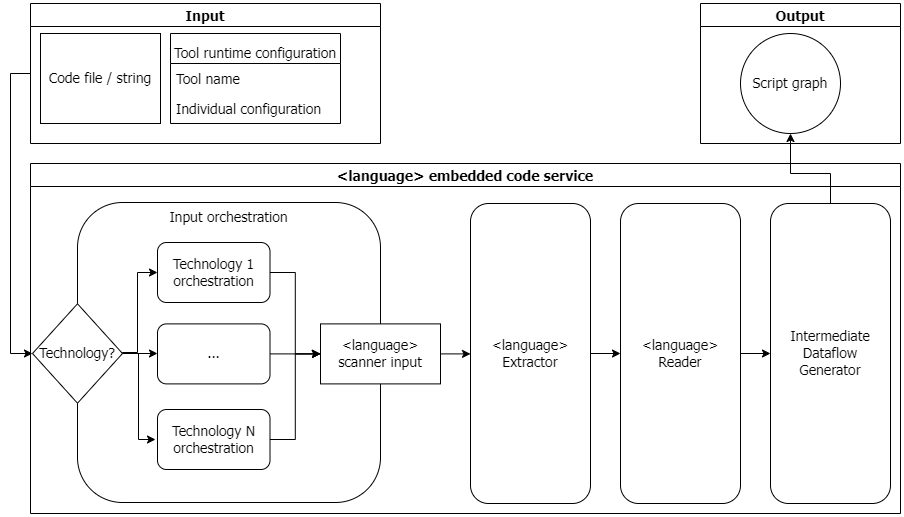
\includegraphics[width=1.0\textwidth]{img/Embedded code service base design.png}
\caption{Diagram of Embedded Code Service workflow}
\label{fig:ECSbasedesign}
\end{figure}   

\subsection{Orchestration}

All contemporary programming languages use some form of import mechanism where the developers can import additional libraries and frameworks. We can see that in embedded code too, often there is a mechanism for adding external libraries to be imported and used by the code. For example in AWS Glue, it is possible to define an argument of an ETL job that specifies an Amazon S3 location of a custom Python library. When AWS Glue executes a Python job, firstly it checks the S3 location and when it conforms to the required format, it copies the files to the internal working directory next to the job script. When the job is started, Python import mechanism is able to find and import these additional libraries to be used in the job script.
\par
Additionally, some technologies (e.g. SAS, Databricks) perform additional orchestration to run the embedded code correctly, such as injecting it in a well-defined class, so this envelope does not have to be written by the user every time, adding the desired imports and only then the embedded code is run on the execution engine used by that technology. This process has to be mimicked by Embedded Code Service before the programming language scanner analyzes the code to provide an equivalent of the actual code that is executed.
\par
The orchestration process would generally be different for each technology and programming language, but there are some common steps and some repeating patterns. This needs to be reflected in the design of orchestration so the part that needs to be implemented anew when the support for a new source technology is added is clearly distinguished from common parts. We can use \textit{template method} design pattern that implements common parts of the process in the base class and lets extending classes redefine the specific parts. That way we clearly define what can and needs to be implemented.

\subsection{Result}

When the analysis of embedded code is finished, the service shall return the result to the source technology scanner. The result is a graph that needs to be merged with another graph and may contain pin nodes that need to be connected. Rather than returning an unfinished graph, we shall return an object that wraps it and provides an interface for connecting pin nodes and merging two graphs. The justification is simple, this graph is not always in a valid state so it should be hidden from plain view and unwanted modifications.

\subsubsection{Pin node mapping}
First thing to be done with the result is pin node mapping. This process was described in Section~\ref{sec:pin}. Pin nodes can be found in the graph by enumerating its nodes and filtering those with pin node type. Each pin node can be distinguished from others by its name.
\par
The source technology scanner performing the mapping should receive the information about created pin nodes from an Insight. A mapping simply contains a pin node and a node to be mapped to. We might want to connect pin nodes by iterating over them and for each one we create a mapping or we might want to iterate over records in an Insight, retrieve the pin node by its name and then create the mapping. Each approach is better in different situations, so the result shall support both operations.
\par
When a mapping is created, it is important to specify whether the pin node is an input node or an output node (relatively to embedded code). The direction decides the orientation of the edge when a pin node is merged to the source technology graph.
\par
During the mapping process, the mapping information is stored and merging is deferred until the end so that the graph remains unchanged throughout the process.

\subsubsection{Merging}
After all pin nodes are mapped, a merge operation can start. This operation can be done only once, because it changes the source technology graph. If it was done multiple times, the graph could be damaged.
\begin{figure}[ht]\centering
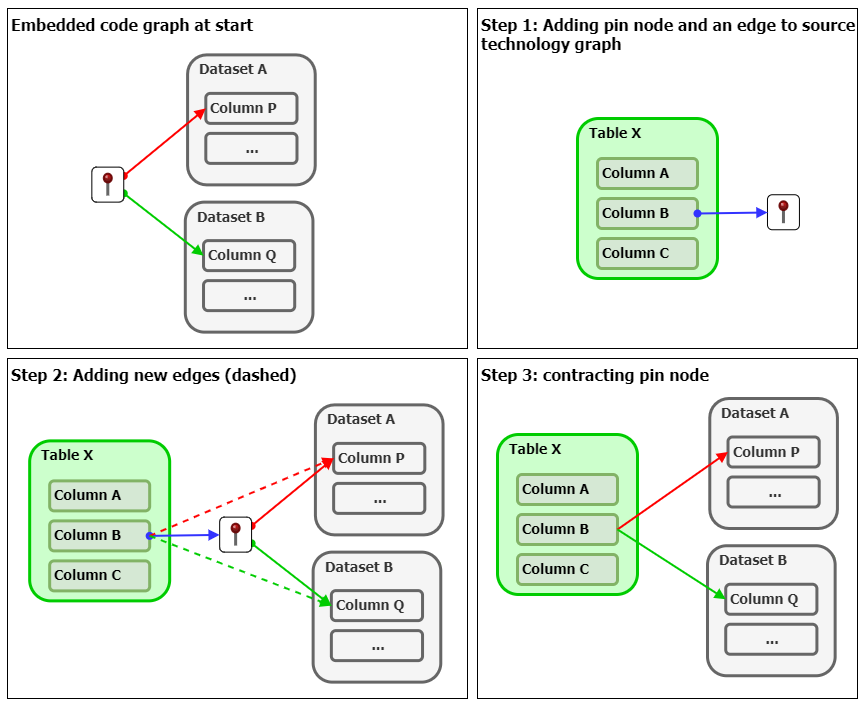
\includegraphics[width=1.0\textwidth]{img/contraction.png}
\caption{The process of merging and contracting a pin node}
\label{fig:contraction}
\end{figure}   
\par
The merging process starts by adding the pin node into the source technology graph along with an edge that connects it to the mapped node. After that, pin node needs to be contracted and removed. That is done by first enumerating its incoming and outgoing edges and adding new edges starting at the starting points of incoming edges and ending at the end points of outgoing edges. After that, pin node and all edges associated with it are removed. A process of contracting a node can be seen in Figure~\ref{fig:contraction}.
\par
When an edge is added to a graph, both its nodes are also added if they were not already present in the graph. After all pin nodes are added to the source technology graph and contracted, all remaining nodes and edges are added and the merging is complete. 

%%----- SECTION -----%% Analysis of Python scanner w.r.t. Embedded Code service
\section{Python scanner changes}

With the design of Embedded Code Service now covered, we need to solve one more issue before we can talk about its implementation. Programming language scanners were not initially designed for running embedded code so we need to review them and design any required changes in order for them to be used in Embedded Code Service. We will be focusing on changes to Python scanner, because in this work we implemented only Embedded Code Service for Python. Other services were not marked as priorities by the stakeholders in scope of this thesis. However, since all programming language scanners follow a very similar design, the changes done on Python scanner may in the future be (with small tweaks) applied also to the remaining scanners.

\subsection{Spring framework}
Before we start with scanner changes, let us have a more detailed look on Manta Flow CLI implementation. It will help us understand some reasons for the changes. Manta Flow CLI is based on the Spring framework. This framework provides a comprehensive set of features and libraries that facilitate the development of robust and scalable Java applications. Among other essential features, we shall look at three of them that we need to understand before following further.
\par
The first important feature is \textit{configuration}. Spring applications typically start with a configuration phase, where developers define the application's beans, dependencies, and other settings. A bean is an object that is managed by Spring. A bean represents a reusable and configurable component of an application. It can be any Java object, ranging from plain Java objects to more complex components. Spring supports two types of configuration, XML-based configuration and Java-based configuration using annotations. Most of the components in Manta Flow CLI use XML-based configuration, however there are several new components in Manta Flow that already use the modern annotation approach.
\par
Second key feature of the Spring framework is its support for \textit{dependency injection}. It allows us to define the dependencies between different components (beans) of the application, and Spring takes care of injecting these dependencies at runtime. This promotes loose coupling and makes the application more modular and easier to maintain.
\par
Lastly, the Spring framework follows the principle of \textit{inversion of control}, which means that the framework is responsible for managing the lifecycle and execution flow of the application. In simpler terms, the application delegates control to the Spring framework, and the framework takes care of executing the appropriate components at the right time.
\begin{figure}[ht]
\begin{lstlisting}[language=Java]
<!-- Define a Spring bean for a simple UserService -->
<bean id="userService" class="com.example.UserService">
   <!-- Inject a dependency using constructor injection -->
   <constructor-arg ref="userRepository" />

   <!-- Set a property value -->
   <property name="maxUsers" value="100" />
</bean>

<!-- Define another Spring bean for UserRepository -->
<bean id="userRepository" class="com.example.UserRepository" />
\end{lstlisting}
\caption{An example of a Spring bean XML configuration and dependency injection}
\label{fig:bean}
\end{figure}
\par
In Figure~\ref{fig:bean} we can see an example of two beans configured in XML: \texttt{userService} and \texttt{userRepository}. The \texttt{userService} bean demonstrates dependency injection by specifying the \texttt{userRepository} bean as a constructor dependency. When the \texttt{userService} bean is created, the Spring container will automatically inject the \texttt{userRepository} bean into it. Additionally, the \texttt{userService} bean showcases property injection by setting the \texttt{maxUsers} property to a value of \texttt{100}. The \texttt{maxUsers} property is assumed to be a property of the \texttt{UserService} class.

%%-subsection-%% 
\subsection{Running the scanner without scenarios}
Each execution of Manta Flow CLI starts a scenario. A scenario consists of a list of tasks required to complete a certain goal. There are many different scenarios, some are used by scanners. for example various extraction and data flow scenarios, some are used for management of metadata repository in Manta Flow Server. Python scanner consists of two scenarios, \textit{Python Extractor Scenario} and \textit{Python Dataflow Scenario}. Extractor scenario is launched to extract input for Python scanner, dataflow scenario performs data flow analysis and generating lineage graph. Each scenario consists of generic code handling startup and completion of a scenario and specific code performing a dedicated task.
\par
Components of Python scanner, Extractor and Reader, as well as Intermediate Dataflow Generator are currently designed specifically to be started and managed by a scenario. It is desired to modify their design and structure to enable starting the scanners from Embedded Code Service. These modifications should not be big (the scanners are already quite well designed), but they need to be finished before a language scanner can be added to the Embedded Code Service.

\subsection{Python scanner design and Spring configuration}
Python Scanner is designed to analyze user inputs. The source code is stored on the file system by users and its location together with other settings is provided in Spring configuration of the scenario when it is launched. Embedded Code Service also receives the source code, but the configuration is different for each input. As Embedded Code Service is also configured only once at the start of a scenario, this configuration has to be built at runtime, specifically in input orchestration phase. 
\par
Upon analyzing the configuration of Python scanner components we can conclude that they were designed as single-purpose components. They are constructed with all functional elements and input configuration that they need to perform their task. Therefore, the lifecycle of such component ends when it finishes its task and a new component has to be constructed for a new task. This is feasible when Python scanner is executed from a scenario, because each scenario executes each task once. With Embedded Code Service the expected lifecycle of components is different. The service is constructed once but can be used for multiple inputs (e.g., analysis of multiple scripts that are a part of one ETL pipeline).
\par
There are two ways how we can modify current components to support both approaches (service and CLI) efficiently. We can modify the component to become stateless. A stateless component does not hold any internal state and can be used repeatedly. Input configuration and state is managed in an instance of a task context class which is passed to the invocation of any method. The context instance can be constructed at runtime or it can be configured as a bean and injected as a dependency. This approach is best suited for components that have a single entry-point - a single method that is invoked to complete the task, but it is not a condition. In such cases the context object is passed as a method parameter during the execution.
\par
The second approach is to create a factory (using \textit{Factory} design pattern) for a component which will be configured in Spring to store the functional elements for the construction of the component (dependencies). The factory will allow passing the input configuration values as parameters to the factory method which constructs a new component. This approach is suitable for components which hold a complex internal state and it would be costly to refactor them to become stateless component. Also, it is a \textit{cheap} modification, there are no changes required in the existing code, we just need to add the implementation of the factory class and this change needs to be reflected in Spring configuration.

\subsection{Interfaces}
We need to consider one more thing. The components were designed to be used by scenarios in Manta Flow CLI and are customized for that purpose. Often their interface contains a single method \texttt{execute} that performs all the steps required by the scenario. Such interface does not provide the functionality we need in Embedded Code Service, because scenarios often require additional tasks to be done that are not required by the service, e.g. serializing connector output on disk. It would be useful to decouple implementation of the functional component from the scenario interface so the functional component can be used by a scenario and Embedded Code Service but it can have its own interface to perform required tasks.

\subsection{Components}
There are three major components in Python scanner: Extractor, Reader and a shared Intermediate Dataflow Generator. These are the components that need to be modified so that they can be used both by scenarios and Embedded Code Service. Let us have a closer look at each of them and the changes that we made.

\subsubsection{Extractor}
Extractor component was already designed in a convenient way. There is a clear separation between the extractor task implementation used in the scenario (implemented in the \texttt{ExtractorTask} class) and the functional component used for the extraction (implemented in the \texttt{Extractor} class). The task uses the functional component to perform the extraction and itself implements all necessary interfaces. The design of the \texttt{Extractor} class almost satisfies our conditions, it is designed as a stateless component with the task context defined in a separate class (\texttt{ExtractorConfiguration}), the only difference is that this context is passed to \texttt{Extractor} instances in the constructor and stored. The context instance does not necessarily need to be stored in the \texttt{Extractor} instance, it was only convenient to do so in the original implementation.
\par
The context contains several file paths pointing to the location of the input or the location of extraction folder that are read-only and need to be available only during the extraction. This component can be easily refactored to conform to the stateless component approach by removing the context from the \texttt{Extractor} class and instead providing it as a parameter to the \texttt{extract} method that performs the extraction. When used in a scenario, the context instance is already stored in the task instance that contains both context and extractor, so there are no Spring configuration changes needed apart from omitting the context as a dependency of an extractor. When used in the service, the context instance can be easily instantiated at runtime using the file paths that the service uses for input orchestration, an extractor will be injected as a dependency of the service.

\subsubsection{Reader}
Python scanner's Reader is a highly state-dependent component. It requires some effort to remove all input-specific information and collect it in a single context instance. Additionally, the current implementation requires refactoring as it does more things than it should. Reader is currently one component that implements both task interface for scenario purposes as well as data flow analysis of Python code done in the scenario.
\par
The increased complexity of the component would make it an ideal candidate to be reworked using the factory approach, but after a deeper analysis we concluded that using this approach would only postpone important changes. The component does two tasks that are demanded by the scenario, but only the analysis needs to be done for embedded code, the other task is serialization of intermediate results for logging and debugging purposes which is not required by Embedded Code Service. Therefore also this interface needs to be fragmented at which point it is worth the time to make a complex refactoring and convert the component to a stateless one. To satisfy all required conditions we need to:
\begin{enumerate}
    \item Decouple task interface from the Reader implementation
    \item Identify stateless functional sub-components of Reader that can be reused 
    \item Identify state information that needs to be stored in a task context instance of Reader
\end{enumerate}
\par
We have split the original \texttt{PythonReader} class implementation into three new classes: \texttt{PythonReader}, \texttt{EntryPointAnalyzer} and \texttt{AnalyzerConfiguration}. \texttt{EntryPointAnalyzer} is a stateless functional component that performs data flow analysis of a single entry point. In Python data flow analysis, an entry point is a module or a function where data flow analysis begins. When analyzing embedded code, there is always only one well-defined entry point, in application analysis there may in general be multiple entry points. This component will be a reusable dependency of both Reader and Embedded Code Service used for analyzing individual entry points. To analyze an entry point, it requires an entry point specification and an analyzer configuration.
\par
\texttt{AnalyzerConfiguration} is a component holding context which is used by \texttt{EntryPointAnalyzer}. It is like a small toolbox that the analyzer uses during the analysis. A new configuration has to be provided for each input, not for each entry point. The reason is that there are certain components that can be shared across multiple entry points of one input to improve performance, such as service for parsing Python code as the code files are common for all entry points, thus they only need to be parsed once. A new analyzer configuration has to be created for each input of Embedded Code Service, only one is required in a scenario.
\par
Lastly, \texttt{PythonReader} class has been modified to work as an implementation of Reader component used by data flow scenario. Internally it uses an entry point analyzer and its own analyzer configuration to analyze all entry points one after the other defined in the input. 
\par
With these modifications, the Spring configuration had to be split in two parts so that the dependencies can be correctly resolved. First one is a general configuration that provides an \texttt{EntryPointAnalyzer} bean. The other is a scenario-specific configuration that creates the \texttt{AnalyzerConfiguration} bean and injects it to a \texttt{PythonReader} bean along with an imported analyzer bean.

\subsubsection{Intermediate Dataflow Generator}
Intermediate Dataflow Generator is a shared component that can be configured and used by any of the programming language scanners. We had to make sure that it keeps this property after all the changes. Generator has been recently refactored and the new implementation already follows many of the principles of a stateless component. However, converting it to a stateless component was not the main focus of the mentioned refactoring so we still need to do a few additional changes. There is a similar problem as in Reader that the \texttt{TransformationTask} class implements both a task for the scenario and generating data lineage graph. By splitting it into two classes, one for the purposes of the scenario and the other for generating data lineage graph, we can easily create a stateless component which can also be used by Embedded Code Service.
\par
After the refactoring, a new \texttt{DataflowGenerator} class is the stateless component of Intermediate Dataflow Generator. \texttt{ProgramConfiguration} is a new class introduced to hold the context information about the input. Lastly, the refactored \texttt{TransformationTask} class is now just the implementation of the scenario task, previously it represented all of these new components.
\par
While these changes of Intermediate Dataflow Generator required little code modifications, it resulted in big changes in its Spring configuration. The Spring configuration of Intermediate Dataflow Generator is layered into multiple levels to introduce modularity. This modularity is important as there are currently 3~programming language scanners that utilize the generator and each of them is slightly different. Moreover, with the introduction of Embedded Code Service, there is another use-case with different needs. The new design reduces the amount of beans that it depends on to a bare minimum and avoids the need to define beans that are unused.
\par
Currently, there are two possible configuration compositions. One is for scanners that are not supported in Embedded Code Service and the other for those that are. For that purpose the configuration of common beans is split in two. Base configuration sets up the stateless functional \texttt{DataflowGenerator} component that can also be used by Embedded Code Service. The other configuration sets up also context beans and scenario task bean that is required for CLI integration. These configurations are then included in scanner-specific configuration that provides scanner-specific beans.
\par
When Embedded Code Service is not implemented for the programming language, the situation is simple as Generator is only used from a scenario, so only the scanner-specific beans need to be provided. In Figure~\ref{fig:generatorNoECS} we can see that the configurations are \textit{layered} one on top of another. Each \textit{layer} creates new beans using the beans provided by the previous one, as seen in \textit{composition} diagram. In \textit{dependencies} diagram we can see what beans the configuration provides to the others and which it depends on. An arrow shows that a bean is available in the configuration at its beginning and is required by the configuration at its end.
\begin{figure}[ht]\centering
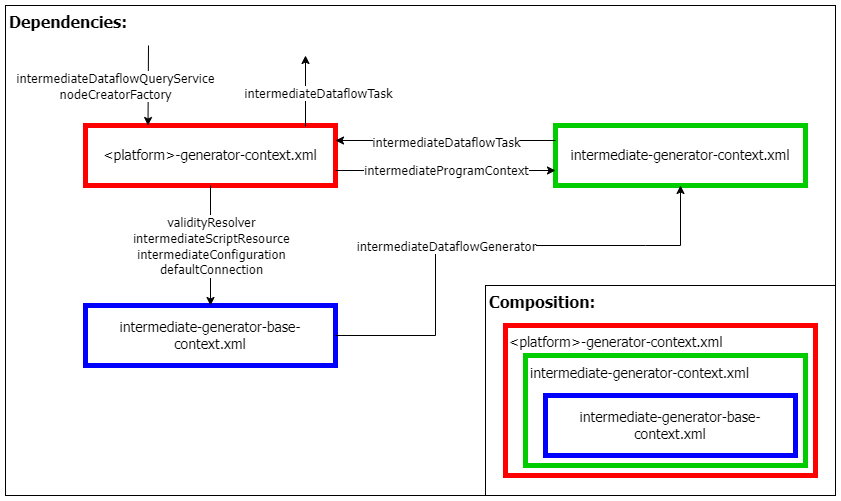
\includegraphics[width=1.0\textwidth]{img/generator_no_ECS.png}
\caption{Composition and dependencies of Generator configurations when Emebedded Code Service is not supported for that programming language scanner}
\label{fig:generatorNoECS}
\end{figure} 
\par
When Embedded Code Service is involved, there needs to be one configuration that satisfies the scenario use-case and there can be another one that satisfies Embedded Code Service needs. Embedded Code Service does not need the scenario beans, in fact, they add useless functionality for such use-case, so its best to avoid it. Moreover, in this use-case there could be multiple program configurations passed to Intermediate Dataflow Generator during its lifecycle which cannot be defined statically in Spring. To satisfy these needs the scanner-specific configuration is split in two parts. First part is the configuration of common beans for both use-cases and then there are two specializations that utilize common beans - scenario (scanner) and service specialization.
\par
Figure~\ref{fig:generatorECS} shows a different, more complex composition of individual configurations. Similarly to the previous case, \textit{dependencies} diagram shows what beans the configuration provides to the others and which it depends on.
\begin{figure}[ht]\centering
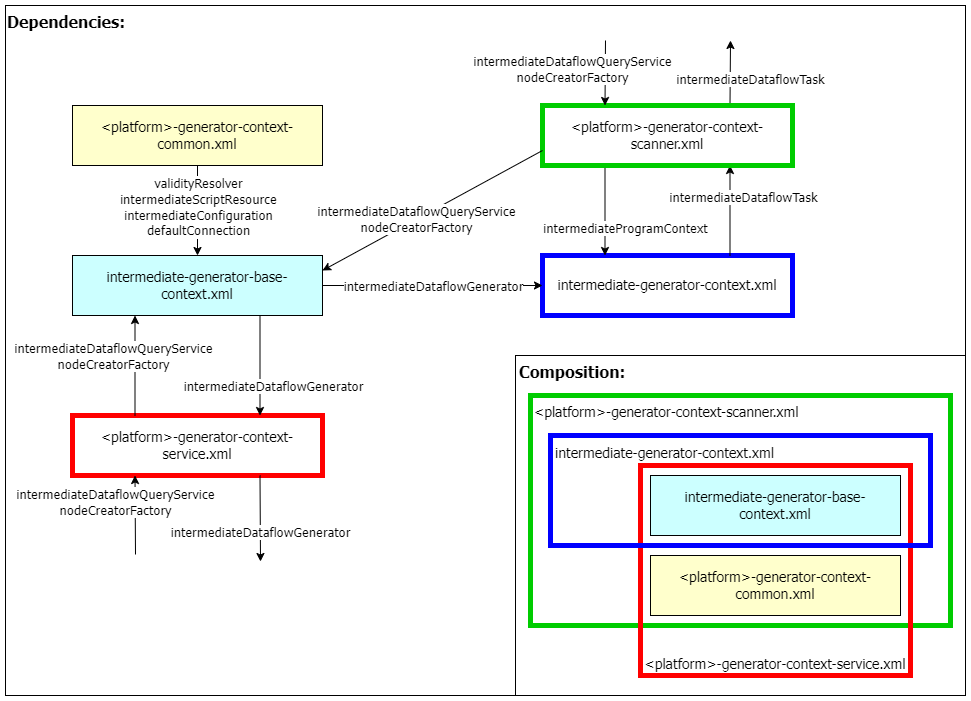
\includegraphics[width=1.0\textwidth]{img/generator_ECS.png}
\caption{Composition and dependencies of Generator configurations when Embedded Code Service is supported for that programming language scanner}
\label{fig:generatorECS}
\end{figure}

\subsection{Insight and Outsight}
There is one more change that we would like to present. Even though it was not implemented as a part of this work, it is a part of the required scanner changes to facilitate its usage in Embedded Code Service, so it makes sense to mention it. We are talking about \textit {Insight and Outsight} mechanism that is used for pin node mapping, but can in general be used to send metadata for embedded code analysis from the source technology scanner as well as to receive additional metadata generated during such analysis to be used by the source technology scanner.

\subsubsection{Insighter}
\textit{Python Insighter} is a way to provide insight to Python code analysis for external consumers. The main idea is to collect events that are important for the external consumer, but which otherwise should not affect Python analysis. Each external consumer has to implement its own Insighter specialization together with collaborative propagation modes needed for the specific data technology. Collaborative propagation modes do not propagate data flows, but instead record events into the specialized Insighter. After the analysis is complete, an immutable \textit{Insight} object is created which contains the recorded events and can be used by an external consumer.
\par
We can categorize events into data events and lineage events. They need to be handled differently based on their category. Data events are events where we need to know an exact data value regardless of its origin, e.g. SQL query, database connection string etc. For the consumer, the concrete value is the important part, which is recorded in the Insight object. Lineage events are the opposite to data events. The exact value is not important in this case, but rather we track these events to create data lineage graph, e.g. reading from a file or a database. The difference from data event is that on top of recording the event into the Insighter, a pin node is created and registered as well. After the analysis ends, the external technology can utilize the recorded information to map pin nodes.

\subsubsection{Outsight}

To propagate external information for Python analysis, we can use the Insighter idea and apply it in a reversed manner. \textit{Outsight} object represents events propagated into the analysis. It can use collaborative propagation modes to convert external events and values into Python data flows. For example, Outsight can be used to create input pins or set values of variables configured in an outside environment.

\begin{figure}[ht]\centering
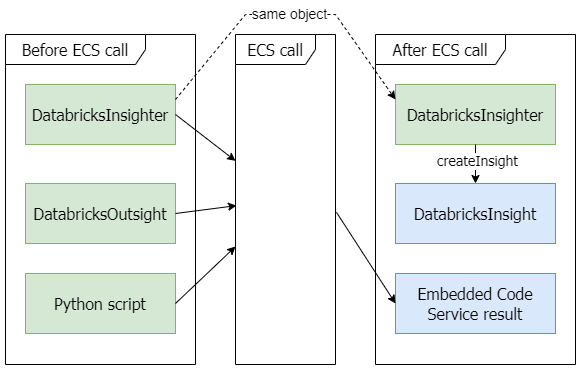
\includegraphics[width=1.0\textwidth]{img/insighter.png}
\caption{Workflow of using Insighter along with Embedded Code Service in Databricks scanner}
\label{fig:insighter}
\end{figure}

\subsubsection{Workflow}

Let us present the workflow of this mechanism as it is used in the scanner for Databricks. This scanner was developed along with Embedded Code Service and uses it for analyzing Python code cells in Databricks notebooks.
\par
Figure~\ref{fig:insighter} shows how Insighter objects are created and used in Databricks scanner when calling Embedded Code Service. Before embedded code is analyzed, Databricks scanner prepares analyzed script and stores any contextual information needed for its analysis in an Outsight object. It also creates a new Insighter. These arguments are passed into the Embedded Code Service call, Insighter and Outsight are a part of configuration. After the call is complete, Embedded Code Service produces a result object. At this point, Databricks scanner can get an Insight object from the Insighter and use it to merge the result into its data lineage graph.

\section{Python Embedded Code Service implementation}

Changes implemented in Python scanner were a direct prerequisite to enable an implementation of Python Embedded Code Service. Without them the service would not be able to run embedded code analysis. Having explained these changes, we can now discuss interesting details of the implementation of this service.
\par
Python Embedded Code Service is implemented as a standalone service intended to analyze Python embedded code. It implements two important steps - orchestrating the input in a digestible format for Python scanner and merging the resulting Python graph into the graph of the source technology. The rest of the process is delegated to Python scanner.

\subsection{Interface}

The interface of Python Embedded Code Service contains only one method: \texttt{getDataflow}. This method consumes name of the script, the content of the script, script parent node and configuration. It returns \texttt{PythonEmbeddedCodeResult} object which contains the data lineage graph of the analyzed script. The purpose of the arguments is explained in the list below:
\begin{itemize}
    \item Name of the script is used for identifying script nodes in the graph and also for debugging purposes.
    \item Contents of the script can be provided in a file or in a string. A typical workflow of a source technology would prepare such scripts during its extraction and store them in files. These files can be directly used as the input or, if they are not Python source files, the code can be provided in a string.
    \item Parent script node is the node that represents the script in the source technology graph. All nodes in the embedded code graph will use this node as their parent for proper identification.
    \item The configuration stores the runtime and environment configuration for the current script. One script could be run in different environments, with different parameters or with additional user-provided libraries. Configuration that changes between scripts (is not same for each script of given technology) can be passed in this parameter. The specialized implementation of configuration only needs to implement a method that tells its kind (for safe type casting), the rest of it can be freely implemented for source technology needs.   
\end{itemize}

\subsection{Result}
The return value of Python Embedded Code Service is implemented in the \texttt{PythonEmbeddedCodeResult} class. It is implemented in a similar fashion as the return value of Dataflow Query Service. It does not provide the result graph directly but instead provides an interface for connecting the two graphs. This interface contains methods for the lookup of pin nodes in the result and creating pin node mappings. After all the mappings are created, we can call the \texttt{mergeTo} method which merges result graph with source technology graph provided as an argument. After this operation, the result is considered to be consumed and cannot be used again.

\subsection{Orchestration}
The orchestration component prepares the input for data flow analysis. This is done in three steps: input orchestration, extraction and processing of the extracted input.
\par
The component is implemented using the \textit{template method} pattern. This pattern allows creating a template for a method where some of its steps can be reimplemented and the rest is constant. The pattern was chosen to encapsulate differences in input preparation for different source technologies into individual classes. The method works as follows:
\begin{enumerate}
    \item Common: a temporary input directory is created. In this directory there is space for preparation of the input for the extractor as well as space for the extractor output.
    \item Specific: input preparation. A specific orchestrator for data technology prepares the input based on the configuration.
    \item Common: the service creates a new Extractor context and runs extraction using Python Extractor and the context. The extracted output is placed in the temporary directory.
    \item Common: the service processes the extracted input by locating the entry point and creating a new analyzer configuration.
\end{enumerate}
\par
Entry point location and analyzer configuration are the outputs of orchestration and are used by entry point analyzer to analyze data flows.

\subsection{Testing}

Python Embedded Code service is covered by a set of unit and integration tests.
\par
Unit tests verify functionality of individual classes, e.g. orchestrators storing files in correct locations or that pin node mapping is done correctly.
\par
Integration tests verify that all components of Python Embedded Code Service are integrated and cooperate correctly. These tests run the service on different inputs and check that the data lineage graph looks as expected after the analysis and merging.
\par
Code coverage by tests reaches 64\% according to SonarQube, a code quality tool used in Manta. This number can be considered lower than standard, but we need to look why that is. The bulk of the uncovered lines are bodies of \texttt{equals} or \texttt{toString} methods along with logging messages which do not require code coverage. In combination with a low amount of code lines in Python Embedded Code Service it results in a lower coverage percentage, but the service can be considered sufficiently covered by tests.